\documentclass[tikz,border=10pt]{standalone}
\usepackage{pgfplots}
\pgfplotsset{compat=1.16}

\begin{document}
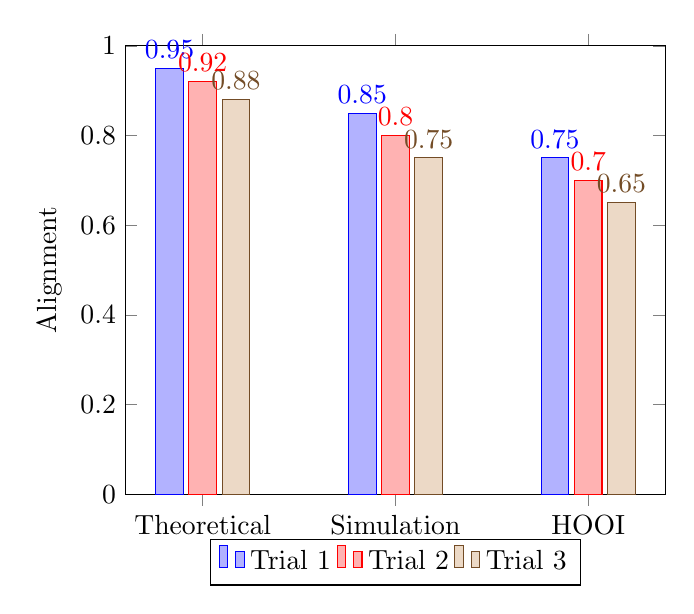
\begin{tikzpicture}
    \begin{axis}[
        ybar,
        symbolic x coords={Theoretical, Simulation, HOOI},
        xtick=data,
        ylabel=Alignment,
        xlabel=Method,
        ymin=0,
        ymax=1,
        enlarge x limits=0.2,
        legend style={at={(0.5,-0.1)}, anchor=north,legend columns=-1},
        nodes near coords,
        nodes near coords align={vertical},
    ]
        \addplot coordinates {(Theoretical,0.95)(Simulation,0.85)(HOOI,0.75)};
        \addplot coordinates {(Theoretical,0.92)(Simulation,0.80)(HOOI,0.70)};
        \addplot coordinates {(Theoretical,0.88)(Simulation,0.75)(HOOI,0.65)};
        \legend{Trial 1, Trial 2, Trial 3};
    \end{axis}
\end{tikzpicture}
\end{document}